\documentclass[ignorenonframetext,xcolor=pdflatex,table,dvipsnames,serif]{beamer}
\usetheme{metropolis} %https://github.com/matze/mtheme

\usepackage[utf8]{inputenc}
\usepackage[english]{babel}
\usepackage{amssymb}
\usepackage{amsmath}
\usepackage{bm}
\usepackage{fancyvrb}
\usepackage{fontawesome5}

\newcommand{\BTheta}{\text{\faBasketballBall}}

\DeclareMathOperator{\E}{\mathbb{E}}
\DeclareMathOperator{\Var}{Var}
\DeclareMathOperator{\Erf}{Erf}
\DeclareMathOperator{\Cov}{Cov}
\DeclareMathOperator{\logit}{logit}
\DeclareMathOperator*{\argsup}{arg\,sup}
\newcommand{\indep}{\perp \!\!\! \perp}
\newcommand\independent{\protect\mathpalette{\protect\independenT}{\perp}}
\def\independenT#1#2{\mathrel{\rlap{$#1#2$}\mkern2mu{#1#2}}}

\title{{\tiny \faBasketballBall} {\scriptsize \faBasketballBall} {\small \faBasketballBall} {\faBasketballBall} {\LARGE \faBasketballBall} {\huge \faBasketballBall} Having A Ball {\huge \faBasketballBall} {\LARGE \faBasketballBall} {\faBasketballBall} {\small \faBasketballBall} {\scriptsize \faBasketballBall} {\tiny \faBasketballBall}}

%\title{{\huge \faBasketballBall} {\LARGE \faBasketballBall} {\faBasketballBall} {\small \faBasketballBall} {\scriptsize \faBasketballBall} {\tiny \faBasketballBall} Having A Ball {\tiny \faBasketballBall} {\scriptsize \faBasketballBall} {\small \faBasketballBall} {\faBasketballBall} {\LARGE \faBasketballBall} {\huge \faBasketballBall}}

\subtitle{\textbf{Evaluating scoring streaks and game excitement using in-match trend estimation}}
\date{March 24th 2021}
\author{Claus Thorn Ekstrøm and Andreas Kryger Jensen}
\institute{Biostatistics, Department of Public Health\\ University of Copenhagen}


%tiny, scriptsize, small, ?, LARGE, huge
\begin{document}

\frame[plain]{\titlepage}
 
\begin{frame}{Roadmap}
  \setbeamertemplate{section in toc}[sections numbered]
  \tableofcontents[hideallsubsections]
\end{frame}
 
%\maketitle

%%%%%%%%%%%%%%%%%%%%%%%%%%%%%%%%%%%%%%%%%%%%%%%%%%%%%%%%%%%%%%%%%%%%%%%%%%%%%%%%%%%%%%%%%%
\section{Introduction}

\begin{frame}[fragile]{How it all started}
\begin{Verbatim}[fontsize=\footnotesize]
Dear sports-analytics-enthusiastic colleagues,

Today I want to make you aware of yet another call for a Special 
Issue on Statistics in Sports in the AStA Advances in Statistical 
Analysis journal (A Journal of the German Statistical Society) 
which Dominik Liebl and I are currently hosting as guest editors:

https://www.springer.com/journal/10182/updates/17805238

We are looking forward to receiving high quality submission 
from at least some of you until 31 October 2020. :-)

All the best, take care and stay safe,
Dominik & Andreas	
\end{Verbatim}
\end{frame}

\begin{frame}{Motivating example}
Game development in the final match of the NBA 2019–2020 season between Los Angeles Lakers and Miami Heat at October 11, 2020. Positive values $\Rightarrow$ LA Lakers are leading.

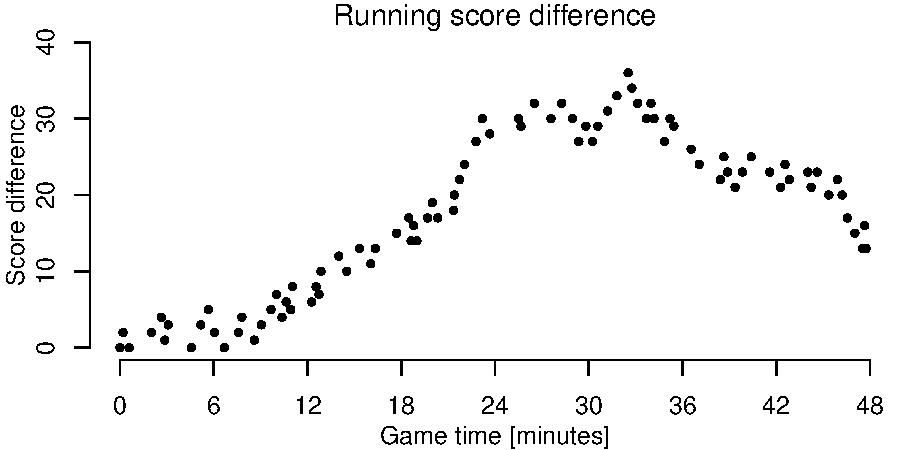
\includegraphics[scale=0.7]{fig1.pdf}

How exciting was this match?
\end{frame}







%%%%%%%%%%%%%%%%%%%%%%%%%%%%%%%%%%%%%%%%%%%%%%%%%%%%%%%%%%%%%%%%%%%%%%%%%%%%%%%%%%%%%%%%%%
\section{Latent dynamics GP Regression}
\begin{frame}{Gaussian Process regression with latent dynamics}
The generative model of GP regression with data $\mathcal{D}_m = \left(D_m(t_{mi}), t_{mi})\right)_{i=1}^{n_m}$ is given hierarchically as
\begin{align*}
\begin{split}
  \BTheta_m \mid \bm{\Psi}_m, \mathbf{t}_m &\sim H(\BTheta_m \mid \bm{\Psi}_m)\\
  d_m(t) \mid \BTheta_m &\sim \mathcal{GP}(\mu_{\bm{\beta}_m}(t), C_{\bm{\theta}_m}(s, t))\\
  D_m(t_{mi}) \mid d_m(t_{mi}), t_{mi}, \BTheta_m &\overset{iid}{\sim} N\left(d_m(t_{mi}), \sigma_{m}^2\right)
\end{split}
\end{align*}

\pause
By linearity of differentiation and the properties of the Gaussian distribution we may augment the latent space as
{
\scriptsize
\begin{align*}
  \begin{bmatrix}d_m(s)\\ d^{\prime}_m(t)\\ d^{\prime\prime}_m(u)\end{bmatrix} \mid \BTheta_m &\sim \mathcal{GP}\left(\begin{bmatrix}\mu_{\bm{\beta}_m}(s)\\ \mu^{\prime}_{\bm{\beta}_m}(t)\\ \mu^{\prime\prime}_{\bm{\beta}_m}(u)\end{bmatrix}, \begin{bmatrix}C_{\bm{\theta}_m}(s, s^\prime) & \partial_2 C_{\bm{\theta}_m}(s, t) & \partial_2^2 C_{\bm{\theta}_m}(s, u)\\ \partial_1 C_{\bm{\theta}_m}(t, s) & \partial_1 \partial_2 C_{\bm{\theta}_m}(t, t^\prime) & \partial_1 \partial_2^2 C_{\bm{\theta}_m}(t, u)\\ \partial_1^2 C_{\bm{\theta}_m}(u, s) & \partial_1^2\partial_2 C_{\bm{\theta}_m}(u, t) & \partial_1^2 \partial_2^2 C_{\bm{\theta}_m}(u, u^\prime)\end{bmatrix}\right)
\end{align*}
}
(if the derivatives exist - no Ornstein-Uhlenbeck for you, Sir!)
\end{frame}


\begin{frame}{Gaussian Process regression with latent dynamics}
Inference about the latent processes is given by the posterior 
{
\scriptsize
\begin{align*}
\begin{bmatrix}d_m(s)\\ d_m^\prime(t)\\ d_m^{\prime\prime}(u)\end{bmatrix} \mid \mathcal{D}_m, \BTheta_m \sim \mathcal{GP}\left(\begin{bmatrix}\mu_{d_m}(s)\\ \mu_{d_m^\prime}(t)\\ \mu_{d_m^{\prime\prime}}(u)\end{bmatrix}, \begin{bmatrix} \Sigma_{d_m}(s, s^\prime) & \Sigma_{d_m d_m^\prime}(s,t) & \Sigma_{d_m d_m^{\prime\prime}}(s,u)\\ \Sigma_{d_m^\prime d_m}(t,s) & \Sigma_{d_m^\prime}(t,t^\prime) & \Sigma_{d_m^\prime d_m^{\prime\prime}}(t,u)\\ \Sigma_{d_m^{\prime\prime} d_m}(u,s) & \Sigma_{d_m^{\prime\prime} d_m^\prime}(u,t) & \Sigma_{d_m^{\prime\prime}}(u,u^\prime)\end{bmatrix}\right)
\end{align*}	
}

\vspace{0.5cm}

\pause
Where the components evaluated at any $\mathbf{t}^\ast$ are given by
{
\tiny
\begin{align*}
  \mu_{d_m}(\mathbf{t}^\ast) &= \mu_{\bm{\beta}_m}(\mathbf{t}^\ast) + C_{\bm{\theta}_m}(\mathbf{t}^\ast, \mathbf{t}_m)\left(C_{\bm{\theta}_m}(\mathbf{t}_m, \mathbf{t}_m) + \sigma^2_m I\right)^{-1}\left(\mathbf{D}_m - \mu_{\bm{\beta}_m}(\mathbf{t}_m)\right)\\
  \mu_{d_m^\prime}(\mathbf{t}^\ast) &= \mu^\prime_{\bm{\beta}_m}(\mathbf{t}^\ast) + \partial_1 C_{\bm{\theta}_m}(\mathbf{t}^\ast, \mathbf{t}_m)\left(C_{\bm{\theta}_m}(\mathbf{t}_m, \mathbf{t}_m) + \sigma^2_m I\right)^{-1}\left(\mathbf{D}_m - \mu_{\bm{\beta}_m}(\mathbf{t}_m)\right) \\
  \mu_{d_m^{\prime\prime}}(\mathbf{t}^\ast) &= \mu^{\prime\prime}_{\bm{\beta}_m}(\mathbf{t}^\ast) + \partial_1^2 C_{\bm{\theta}_m}(\mathbf{t}^\ast, \mathbf{t}_m)\left(C_{\bm{\theta}_m}(\mathbf{t}_m, \mathbf{t}_m) + \sigma^2_m I\right)^{-1}\left(\mathbf{D}_m - \mu_{\bm{\beta}_m}(\mathbf{t}_m)\right)\\
  \Sigma_{d_m}(\mathbf{t}^\ast, \mathbf{t}^\ast) &= C_{\bm{\theta}_m}(\mathbf{t}^\ast, \mathbf{t}^\ast) - C_{\bm{\theta}_m}(\mathbf{t}^\ast, \mathbf{t}_m)\left(C_{\bm{\theta}_m}(\mathbf{t}_m, \mathbf{t}_m) + \sigma^2_m I\right)^{-1} C_{\bm{\theta}_m}(\mathbf{t}_m, \mathbf{t}^\ast)\\
  \Sigma_{d_m^\prime}(\mathbf{t}^\ast, \mathbf{t}^\ast) &= \partial_1\partial_2C_{\bm{\theta}_m}(\mathbf{t}^\ast, \mathbf{t}^\ast) - \partial_1C_{\bm{\theta}_m}(\mathbf{t}^\ast, \mathbf{t}_m)\left(C_{\bm{\theta}_m}(\mathbf{t}_m, \mathbf{t}_m) + \sigma^2_m I\right)^{-1} \partial_2C_{\bm{\theta}_m}(\mathbf{t}_m, \mathbf{t}^\ast)\\
  \Sigma_{d_m^{\prime\prime}}(\mathbf{t}^\ast, \mathbf{t}^\ast) &= \partial_1^2\partial_2^2 C_{\bm{\theta}_m}(\mathbf{t}^\ast, \mathbf{t}^\ast) - \partial_1^2 C_{\bm{\theta}_m}(\mathbf{t}^\ast, \mathbf{t}_m)\left(C_{\bm{\theta}_m}(\mathbf{t}_m, \mathbf{t}_m) + \sigma^2_m I\right)^{-1} \partial_2^2 C_{\bm{\theta}_m}(\mathbf{t}_m, \mathbf{t}^\ast)\\
  \Sigma_{d_m d_m^\prime}(\mathbf{t}^\ast, \mathbf{t}^\ast) &= \partial_2 C_{\bm{\theta}_m}(\mathbf{t}^\ast, \mathbf{t}^\ast) - C_{\bm{\theta}_m}(\mathbf{t}^\ast, \mathbf{t}_m)\left(C_{\bm{\theta}_m}(\mathbf{t}_m, \mathbf{t}_m) + \sigma^2_m I\right)^{-1} \partial_2 C_{\bm{\theta}_m}(\mathbf{t}_m, \mathbf{t}^\ast)\\
  \Sigma_{d_m d_m^{\prime\prime}}(\mathbf{t}^\ast, \mathbf{t}^\ast) &= \partial_2^2 C_{\bm{\theta}_m}(\mathbf{t}^\ast, \mathbf{t}^\ast) - C_{\bm{\theta}_m}(\mathbf{t}^\ast, \mathbf{t}_m)\left(C_{\bm{\theta}_m}(\mathbf{t}_m, \mathbf{t}_m) + \sigma^2_m I\right)^{-1} \partial_2^2 C_{\bm{\theta}_m}(\mathbf{t}_m, \mathbf{t}^\ast)\\
  \Sigma_{d_m^\prime d_m^{\prime\prime}}(\mathbf{t}^\ast, \mathbf{t}^\ast) &= \partial_1 \partial_2^2 C_{\bm{\theta}_m}(\mathbf{t}^\ast, \mathbf{t}^\ast) - \partial_1 C_{\bm{\theta}}(\mathbf{t}^\ast, \mathbf{t}_m)\left(C_{\bm{\theta}_m}(\mathbf{t}_m, \mathbf{t}_m) + \sigma^2_m I\right)^{-1} \partial_2^2 C_{\bm{\theta}_m}(\mathbf{t}_m, \mathbf{t}^\ast)
\end{align*}
}
\end{frame}


\begin{frame}{Trend Direction Index (TDI)}
\begin{align*}
\begin{split}
  \textrm{TDI}_m(t \mid \BTheta_m) &= P\left(d_m^\prime(t) > 0 \mid \mathcal{D}_m, \BTheta_m\right)\\
     &= \frac{1}{2} + \frac{1}{2}\Erf\left(\frac{\mu_{d_m^\prime}(t)}{2^{1/2}\Sigma_{d_m^\prime}(t, t)^{1/2}}\right)
\end{split}
\end{align*}	
\end{frame}

\begin{frame}{Excitement Trend Index}
\begin{align*}
\begin{split}
  \text{ETI}_m \mid \BTheta_m &= \E\left[\#\left\{t \in \mathcal{I}_m : d^\prime_m(t) = 0\right\} \mid \mathcal{D}_m, \BTheta_m\right]\\
  &= \int_{\mathcal{I}_m} \int_{-\infty}^\infty \left|v\right| f_{d^\prime_m(t), d^{\prime\prime}_m(t)}(0, v \mid \mathcal{D}_m, \BTheta_m)\textrm{d}v\textrm{d}t \\
  &= \int_{\mathcal{I}_m} d\mathrm{ETI}_m(t \mid \BTheta_m)\mathrm{d}t
\end{split}
\end{align*}	
\end{frame}


\begin{frame}{Excitement Trend Index}
?
{
\small
\begin{align*}
d\mathrm{ETI}_m(t \mid \BTheta_m) = \lambda_m(t)\phi\left(\frac{\mu_{d_m^\prime}(t)}{\Sigma_{d_m^\prime}(t,t)^{1/2}}\right)\left(2\phi\left(\zeta_m(t)\right) + \zeta_m(t)\Erf\left(\frac{\zeta_m(t)}{2^{1/2}}\right)\right)
\end{align*}
}

{
\small
\begin{gather*}
  \lambda_m(t) = \frac{\Sigma_{d_m^{\prime\prime}}(t,t)^{1/2}}{\Sigma_{d_m^\prime}(t,t)^{1/2}}\left(1-\omega_m(t)^2\right)^{1/2}, \quad \omega_m(t) = \frac{\Sigma_{d_m^\prime d_m^{\prime\prime}}(t,t)}{\Sigma_{d_m^\prime}(t,t)^{1/2}\Sigma_{d_m^{\prime\prime}}(t,t)^{1/2}}\\
  \zeta_m(t) = \frac{\mu_{d_m^\prime}(t)\Sigma_{d_m^{\prime^\prime}}(t,t)^{1/2}\omega_m(t)\Sigma_{d_m^\prime}(t,t)^{-1/2} - \mu_{d_m^{\prime\prime}}(t)}{\Sigma_{d_m^{\prime\prime}}(t,t)^{1/2}\left(1 - \omega_m(t)^2\right)^{1/2}}
\end{gather*}
}
\end{frame}

\begin{frame}{Estimation}
\begin{align*}
  \mu_{\bm{\beta}_m}(t) = \beta_m, \quad C_{\bm{\theta}_m}(s, t) = \alpha^2_m\exp\left(-\frac{(s-t)^2}{2\rho^2_m}\right)
\end{align*}

The hyper-parameters are given the following prior distribution
\begin{align*}
H(\BTheta_m \mid \bm{\Psi}_m) = H(\beta_m \mid \Psi_{\beta_m})H(\alpha_m \mid \Psi_{\alpha_m})H(\rho_m \mid \Psi_{\rho_m})H(\sigma_m \mid \Psi_{\sigma_m})
\end{align*}
with
{
\footnotesize
\begin{align*}
\beta_{m} \sim T_4\left(\widehat{\beta_m^\text{ML}}, 5\right), \; \alpha_m \sim T^+_4\left(\widehat{\alpha_m^\text{ML}}, 5\right), \; \rho_m \sim T_4^+\left(\widehat{\rho_m^\text{ML}}, 5\right), \; \sigma_m \sim T^+_4\left(\widehat{\sigma_m^\text{ML}}, 5\right)
\end{align*}
} 

Super-script ML indicates the marginal maximum-likelihood estimate (empirical Bayes).
\end{frame}

\begin{frame}{Empirical bayes}
To find the empirical Bayes estimate of the hyper-parameters we maximize the marginal log-likelihood function. This can be written as
{
\footnotesize
\begin{align*}
\log L(\BTheta_m \mid \mathcal{D}_m) &\propto - \frac{1}{2}\log |C_{\bm{\theta}_m}(\mathbf{t}_m, \mathbf{t}_m) + \sigma_m^2 I|\\
&- \frac{1}{2}(\mathbf{D}_m - \mu_{\bm{\beta}_m}(\mathbf{t}_m))^T\left[C_{\bm{\theta}_m}(\mathbf{t}_m, \mathbf{t}_m) + \sigma_m^2 I\right]^{-1}(\mathbf{D}_m - \mu_{\bm{\beta}_m}(\mathbf{t}_m))
\end{align*}	
} 

The solution $\widehat{\BTheta_m^\text{ML}} = \argsup_{\BTheta} \log L(\BTheta \mid \mathcal{D}_m)$ can be obtained by numerical optimization.

Our model is implemented in Stan and for each match we ran 4 chains for 50,000 iterations with half of them for warm-up. Output: 2292 gigabyes of posterior data.
\end{frame}


%%%%%%%%%%%%%%%%%%%%%%%%%%%%%%%%%%%%%%%%%%%%%%%%%%%%%%%%%%%%%%%%%%%%%%%%%%%%%%%%%%%%%%%%%%
\section{The 2019--2020 NBA season}

\begin{frame}{The 2019--2020 NBA season}
We applied our method for all 1143 matches from the 2019--2020 NBA basketball season.

We disregarded overtime.
\end{frame}

\begin{frame}{Final match between LA Lakers and Miami Heat}
Analysis of the motivating example.
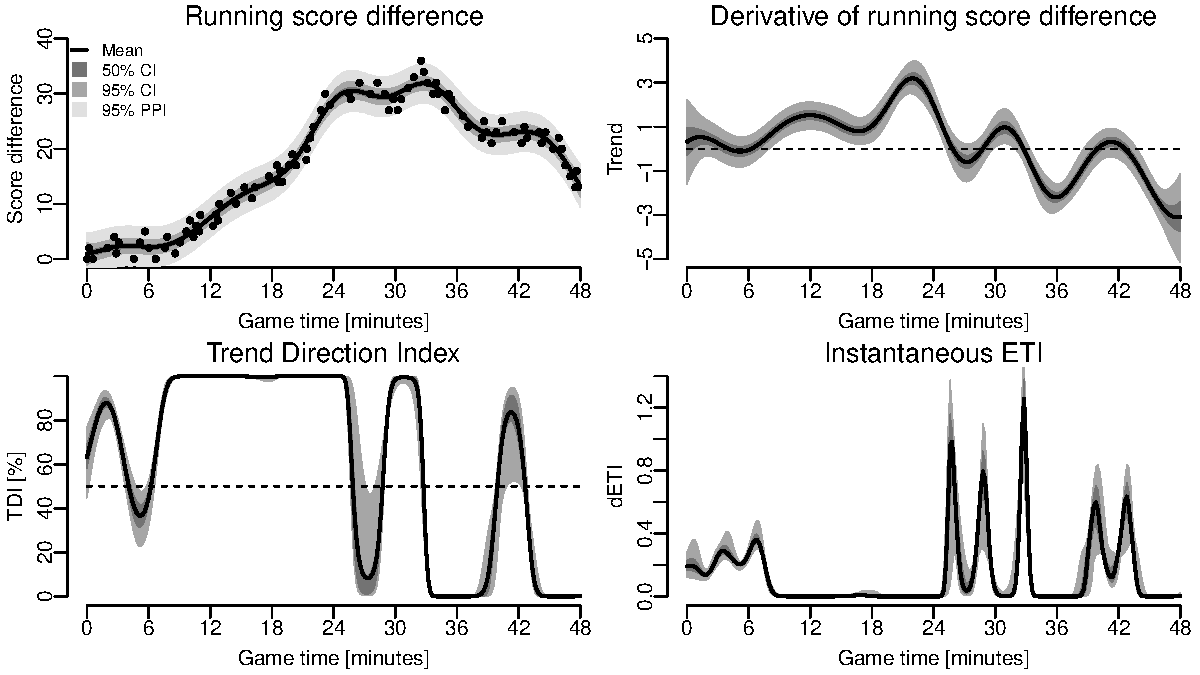
\includegraphics[scale=0.5]{fig2.pdf}
\end{frame}

\begin{frame}{Distribution of the 1143 median posterior ETIs}
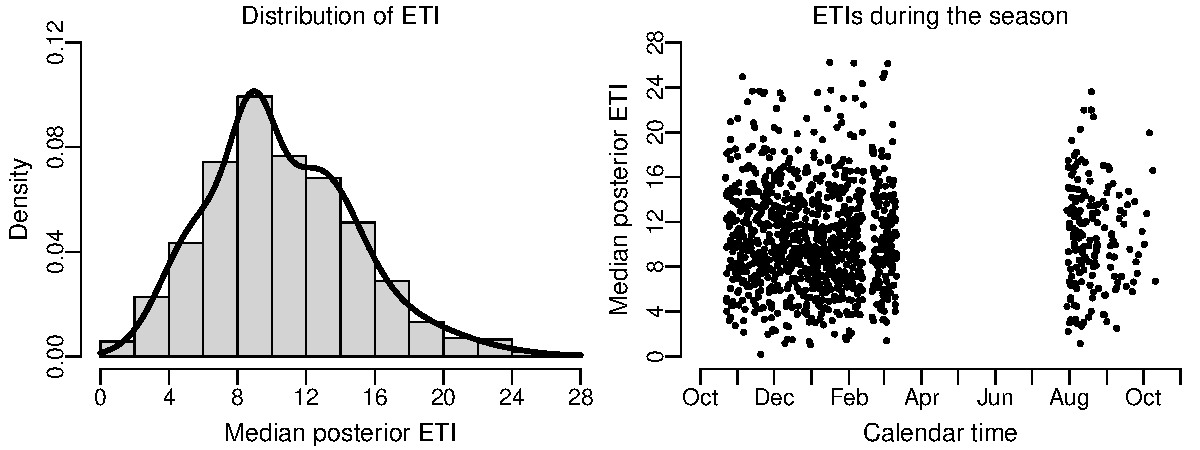
\includegraphics[scale=0.5]{fig3.pdf}
\end{frame}

\begin{frame}{Season minimum ETI}
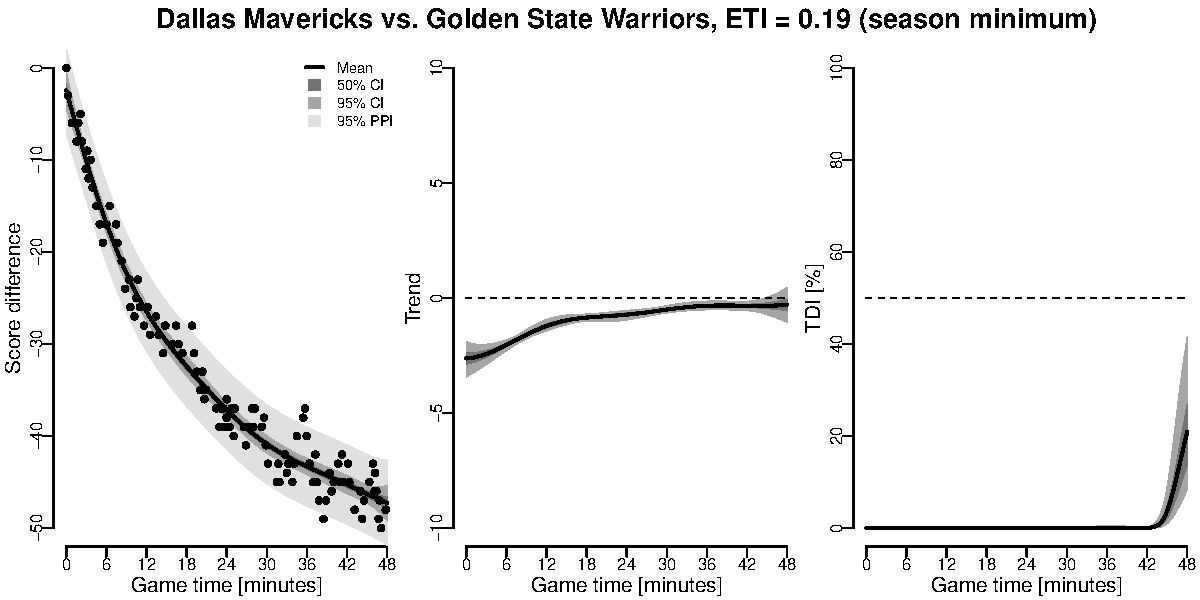
\includegraphics[scale=0.5]{fig4_1.pdf}
\end{frame}

\begin{frame}{Season 25\% percentile ETI}
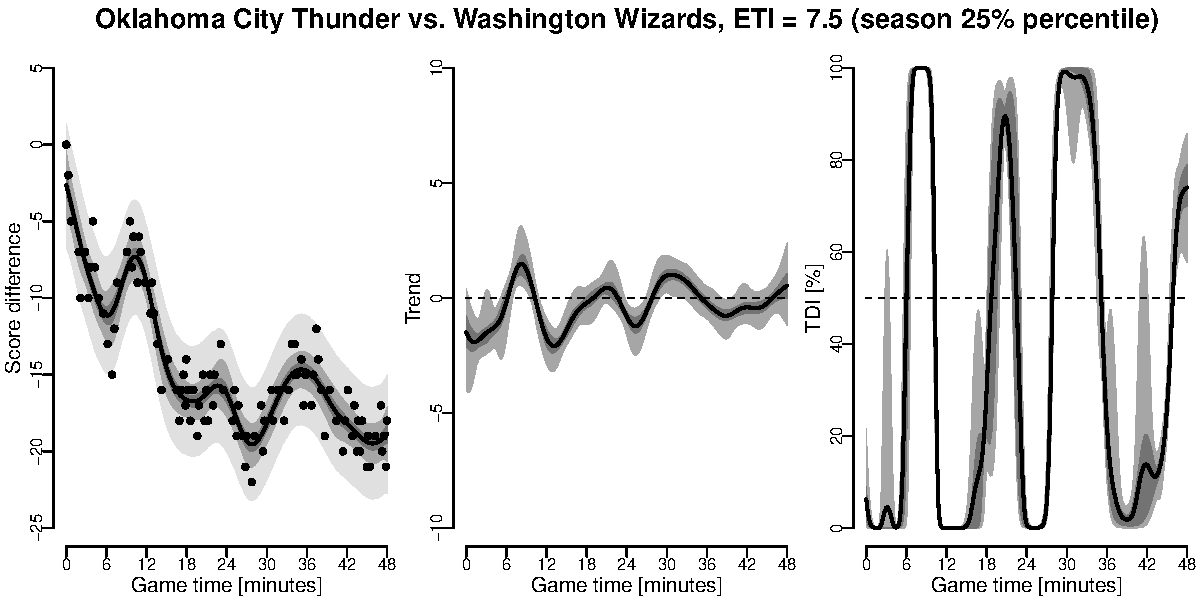
\includegraphics[scale=0.5]{fig4_2.pdf}
\end{frame}

\begin{frame}{Season median ETI}
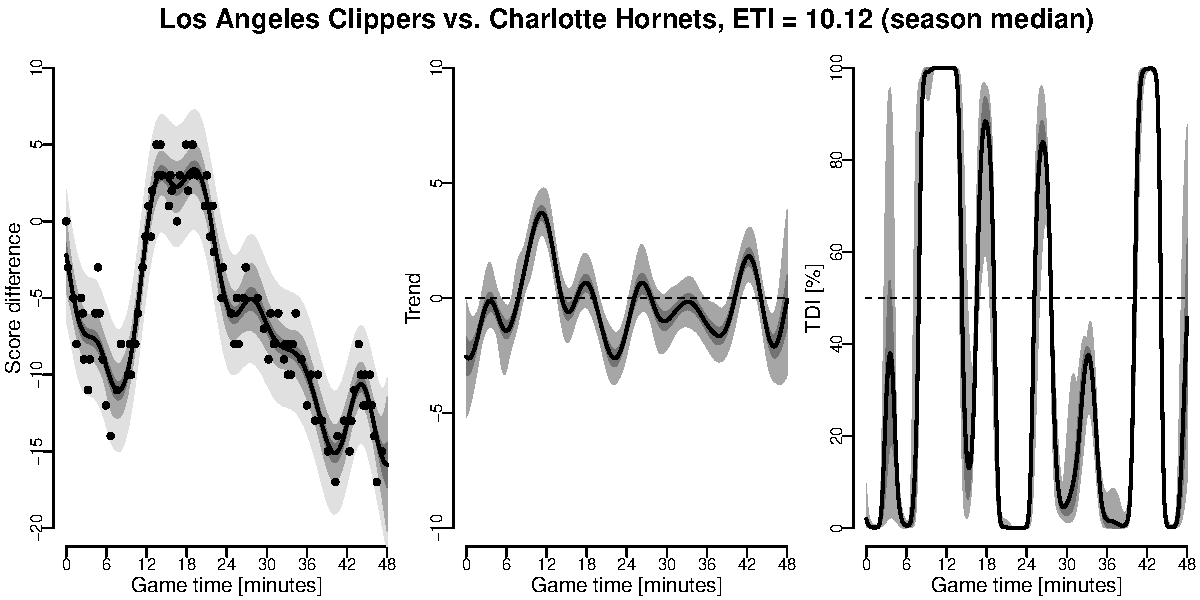
\includegraphics[scale=0.5]{fig4_3.pdf}
\end{frame}

\begin{frame}{Season 75\% percentile ETI}
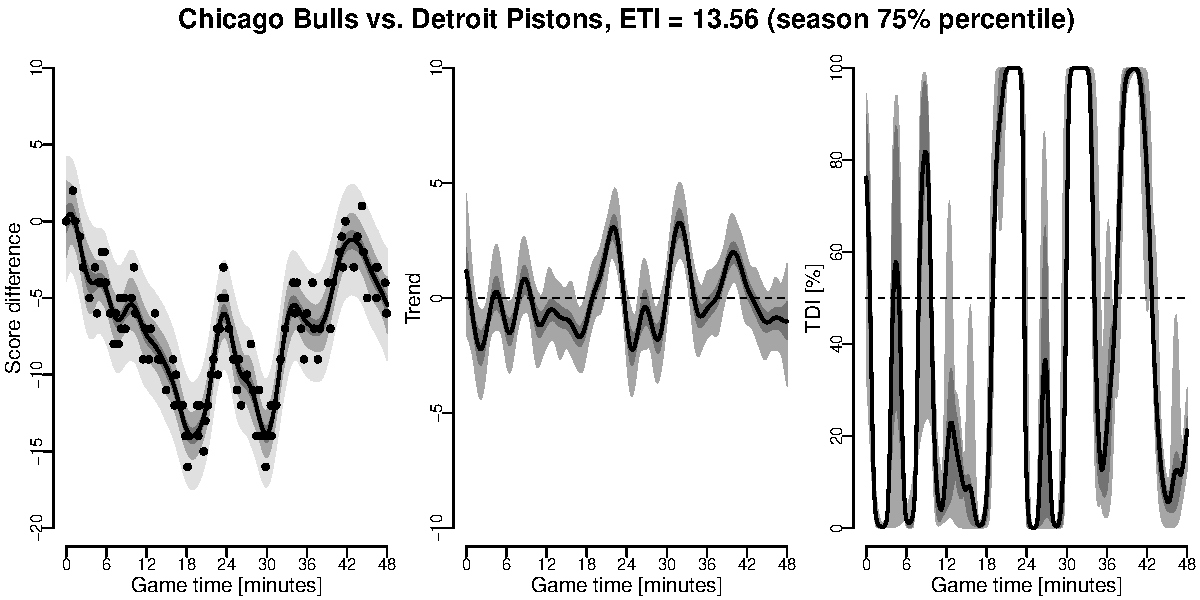
\includegraphics[scale=0.5]{fig4_4.pdf}
\end{frame}

\begin{frame}{Season maximum ETI}
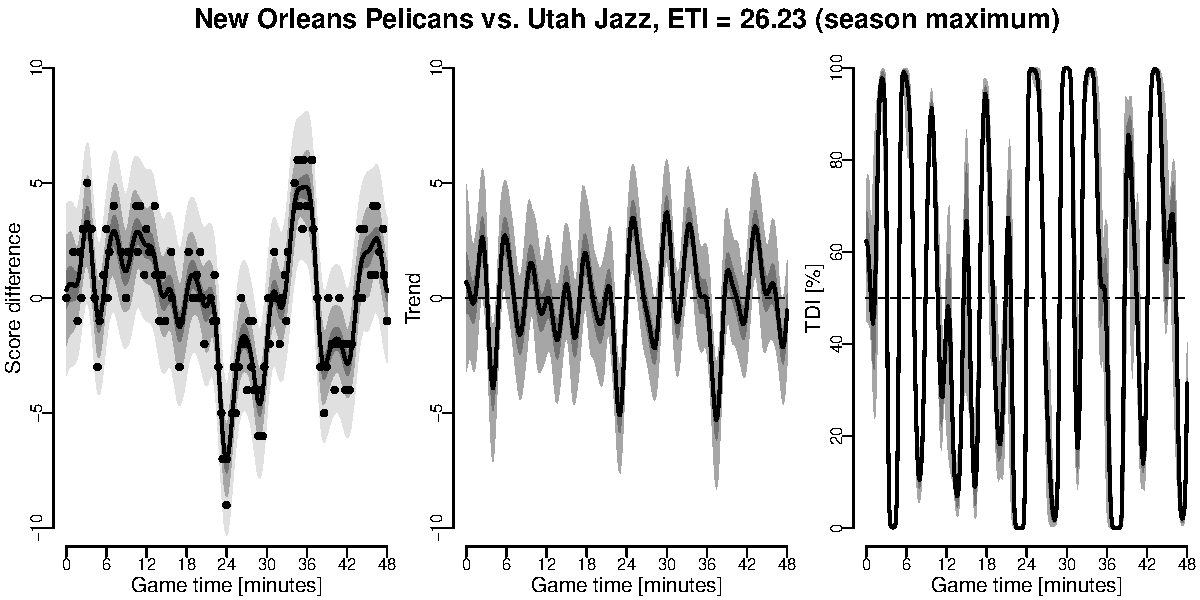
\includegraphics[scale=0.5]{fig4_5.pdf}
\end{frame}



\begin{frame}{An algorithm for collapsing a factor into sub-groups}

  If I were to go see an exciting match --- who should I watch?

  \pause

  Cluster teams based on their median posterior ETI. 

  Compute the $\text{RMSEP}_\text{LOO-CV}^{C=c}$ where $c$ is the number
  of subgroups considering all possible partitions of the 30 teams.
  Essentially a bunch of one-way ANOVAs


  $\text{RMSEP}_\text{LOO-CV}^{C=2} = 4.493$

  $\text{RMSEP}_\text{LOO-CV}^{C=3} = 4.49$

  $\text{RMSEP}_\text{LOO-CV}^{C=4} = 4.489$

  $\text{RMSEP}_\text{LOO-CV}^{C=5+} = 4.489$

  
\end{frame}


\begin{frame}{Clustering results}
\center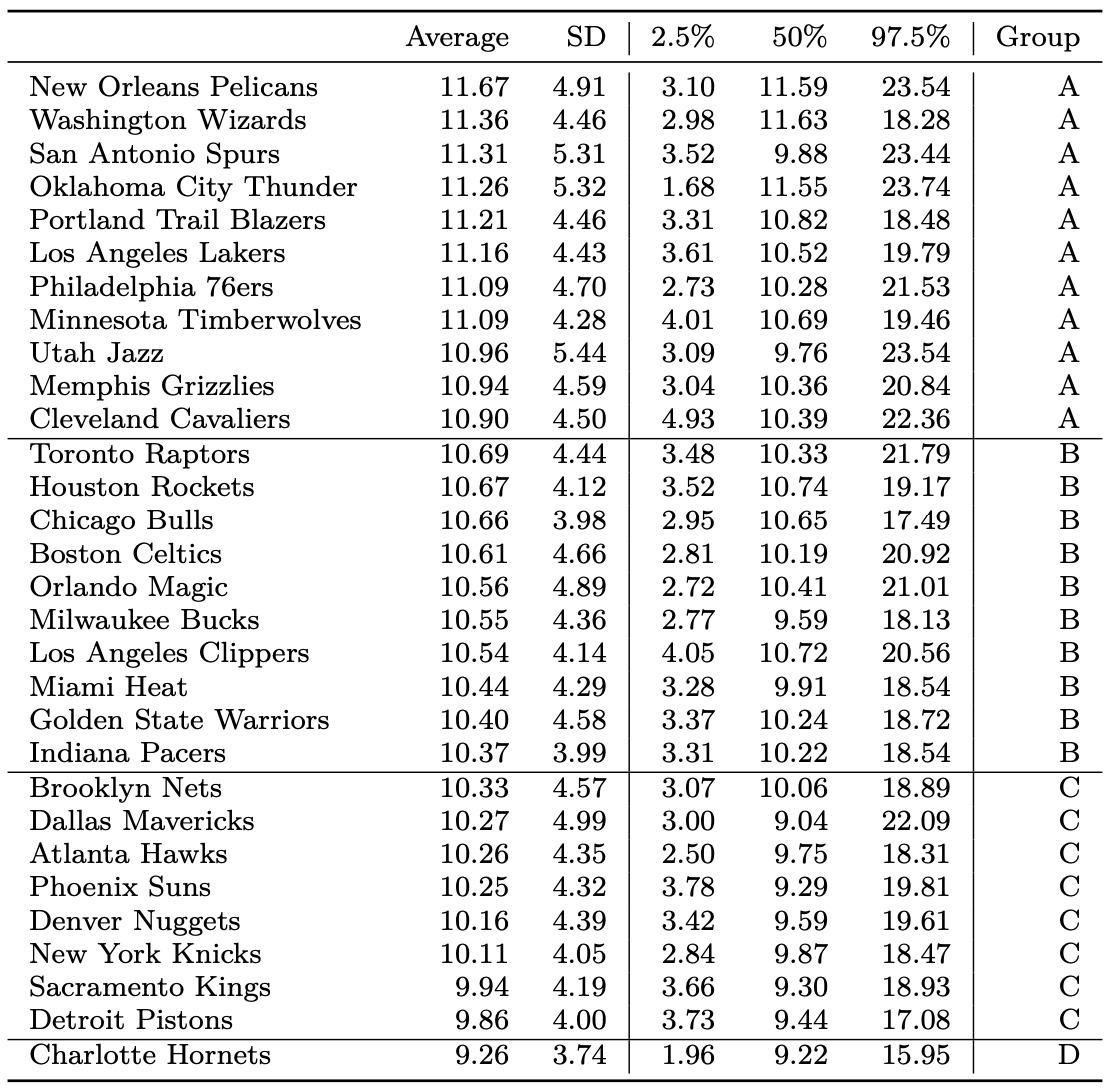
\includegraphics[scale=0.4]{tab1.png}
\end{frame}

\begin{frame}{Team specific seasonal SD vs. average ETIs}
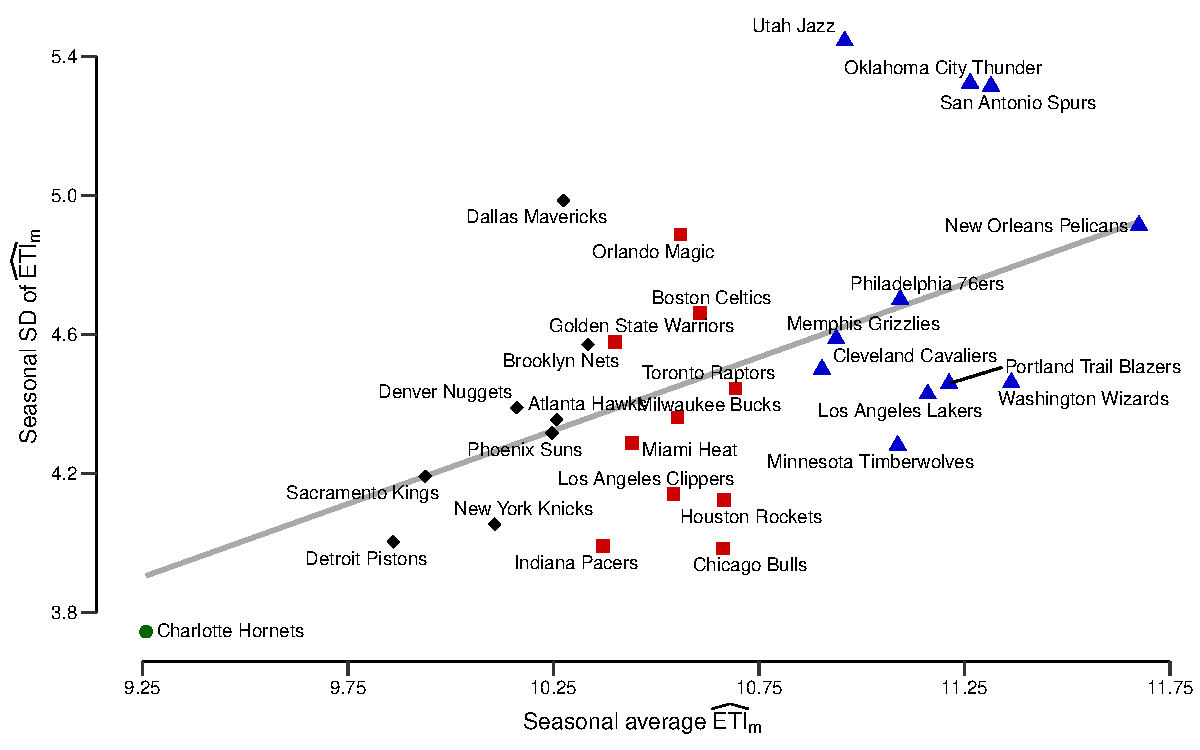
\includegraphics[scale=0.5]{fig5.pdf}
\end{frame}

%%%%%%%%%%%%%%%%%%%%%%%%%%%%%%%%%%%%%%%%%%%%%%%%%%%%%%%%%%%%%%%%%%%%%%%%%%%%%%%%%%%%%%%%%%
\section{Conclusion}

\begin{frame}{Conclusion}

  \begin{itemize}
  \item The trender enables in-game and postgame evaluations about the underlying trends in scoring patterns.
    \item ETI is the expected number of monotonicity changes --- which team appears stronger. High numbers good.
  \end{itemize}

  Future ideas:
  
  \begin{itemize}
    \item Use a weighted ETI to weigh the ETI higher towards the end of the game --- or lower if one team is far ahead.
  \end{itemize}


  Also: have cemented our position as sports-analytics-enthusiasts.
  
\end{frame}



\end{document}
